\documentclass[%
a4paper,
twoside,
openany,
dvipsnames
]
{report}
%
%----------------------------------------------------------------------------
%
% Title
%
\title{Real time face verification using a Zynq-7000-20 FPGA}
%
%----------------------------------------------------------------------------
%
% Author
%
\author{Lukas Baischer}
%
%----------------------------------------------------------------------------
%
% Matrikelnummer/Registrationnumber
%
\newcommand{\registrationnumber}{01426506}
%
%----------------------------------------------------------------------------
%
% Supervisor(s)
%
\newcommand{\supervisor}{Assistant Prof. Nima Taherinejad , PhD}
%
%----------------------------------------------------------------------------
%
% Submission Date
%
\newcommand{\submissiondate}{20.12.2021}

%
% ----------------------------------------------------------------------------
%
% Uncomment only one of the following depending on your type of document:
%
\newcommand{\doctype}{REPORT}
%\newcommand{\doctype}{DISSERTATION}
%\newcommand{\doctype}{MASTERTHESIS}
%\newcommand{\doctype}{BACHELORTHESIS}
%
%-----------------------------------------------------------------------------
%
% Use the 'Libertine' font type
%
\usepackage{libertine}
\usepackage[T1]{fontenc}
\usepackage[utf8]{inputenc}
\usepackage[english,ngerman]{babel}
%
%----------------------------------------------------------------------------
%
% Set page margins
%
\usepackage{geometry}
\geometry{%
	left   = 2cm,
	right  = 2cm,
	top    = 2cm,
	bottom = 2cm
}
%
%----------------------------------------------------------------------------
%
% Set line spacing
%
\usepackage{setspace}
\setstretch{1.5}
%
%----------------------------------------------------------------------------
%
% Set paragraph: No indentation, but include an empty line
%
\usepackage[parfill]{parskip}
%
%----------------------------------------------------------------------------
%
% Settings for hyperlinks
%
\usepackage{hyperref}
\hypersetup{%
	colorlinks = false,
	allcolors  = blue,
}
%
%----------------------------------------------------------------------------
%
% Use graphics
%
\usepackage{graphicx}
\usepackage{subcaption }
%
%----------------------------------------------------------------------------
%
% Use colors
%
\usepackage{xcolor}
\usepackage{colortbl}
%
%----------------------------------------------------------------------------
%
% Define a TODO and a DONE command
%
\newcommand{\todo}[1]{\textcolor{red}{#1}}
\newcommand{\done}[1]{}
%
%
\usepackage[hang]{footmisc}
\renewcommand{\hangfootparindent}{2em}
\renewcommand{\hangfootparskip}{2em}
\renewcommand{\footnotemargin}{0.00001pt}
\renewcommand{\footnotelayout}{\hspace{2em}}
%
%
%----------------------------------------------------------------------------
%
% Set line spacing for all figure environments
% From: https://tex.stackexchange.com/a/166458
%
\let\svfigure\figure
\let\svendfigure\endfigure
\renewenvironment{figure}[1][tb]{\svfigure[#1]\setstretch{1}}
{\svendfigure}
%
%----------------------------------------------------------------------------
%
% Use AMS math fonts
%
\usepackage{amsfonts}
\usepackage[sans]{dsfont}
%
%----------------------------------------------------------------------------
%
% Use multiple figures in one float
%
\usepackage{subcaption}
%
%----------------------------------------------------------------------------
%
% Use dummy text
%
\usepackage{lipsum}
%
%----------------------------------------------------------------------------
%
% Use extended list environments (e.g., 'inparaenum')
%
\usepackage{paralist}
%
%----------------------------------------------------------------------------
%
% Use listings
%
\usepackage{listings}
%
%----------------------------------------------------------------------------
%
% Typeset pseudo code
%
\usepackage{syntax}
%
%----------------------------------------------------------------------------
%
% More options for boxes
%
\usepackage{realboxes}
%
% Command for vertical text in tabulars
%
\newcommand*\rot{\rotatebox{90}}
%
%----------------------------------------------------------------------------
%
% Package for logos (e.g., the BibTeX logo)
%
\usepackage{dtk-logos}
%
%----------------------------------------------------------------------------
%
% Use \textsubscript
%
\usepackage{fixltx2e}
%
%----------------------------------------------------------------------------
%
% More options for tabulars
%
\usepackage{array}
%
%----------------------------------------------------------------------------
%
% Use appendices
%
\usepackage[titletoc]{appendix}
%
%----------------------------------------------------------------------------
%
% Macros to use title and author information in the document
%
\makeatletter
\let\thetitle\@title
\let\theauthor\@author
\makeatother
%
%----------------------------------------------------------------------------
%
% Do not show page numbers on empty pages
%
\usepackage{emptypage}
%
%---------------------------------------------------------------------------
%
% Set spacing between items (looks really weird otherwise)
\usepackage{enumitem}
\setitemize{itemsep=-8pt}
\setenumerate{itemsep=-8pt}
%
%----------------------------------------------------------------------------
%
% Use algorithm and algpseudocode to create pseudo code algorithms 
%
\usepackage{algorithm} 
\usepackage{algpseudocode} 
%----------------------------------------------------------------------------
%
% Use pythonhighlight for python syntax highlighting see https://github.com/olivierverdier/python-latex-highlighting for more information
%
\usepackage{pythonhighlight}
%
%----------------------------------------------------------------------------
%
% Use svg package for plotting inkscape graphics 
%
\usepackage{svg}
%
%----------------------------------------------------------------------------
% 
% Use float to be able to force figure position using [H]
%
\usepackage{float}
%
%----------------------------------------------------------------------------
% 
% Use pdfpages to be able to add pdf to appendix and pdflscape for landcape pdfs 
%
\usepackage{pdfpages}
\usepackage{pdflscape}
%
%----------------------------------------------------------------------------
% 
% Use glossaries to use acronyms and symbols 
%
\usepackage[acronym,nonumberlist,nowarn,style=long]{glossaries}
\usepackage{makeidx}
\usepackage{csquotes}
%
%----------------------------------------------------------------------------
% 
% For Si units 
%
\usepackage{siunitx}
%
%----------------------------------------------------------------------------
% 
% Box for for research question 
%
\usepackage{fbox}
%
%----------------------------------------------------------------------------
% 
% For nicer tables 
%
\usepackage{booktabs}
\usepackage{tabularx}
\newcolumntype{C}{>{\centering\arraybackslash}X} 
\usepackage{multirow}
%
%----------------------------------------------------------------------------
%
% For section comments 
%
\usepackage{comment}
%
%----------------------------------------------------------------------------
% 
% cite in order to sort citation numbers  
%
\usepackage{cite}
%
%----------------------------------------------------------------------------
%
% Use the cleverref package -- Load this package as the very last!
%
\usepackage{nameref}
%
%----------------------------------------------------------------------------
%
% Use the cleverref package -- Load this package as the very last!
%
\usepackage{cleveref}
%
%----------------------------------------------------------------------------
%
% Include listings for Code highlighting 
%


\definecolor{mygreen}{RGB}{0,102,0} % color values Red, Green, Blue
\definecolor{mylilas}{RGB}{170,55,241}
\definecolor{myred}{RGB}{94,32,40}

%----------------------------------------------------------------------------
% Matlab
\lstset{language=Matlab,%
    %basicstyle=\color{red},
    frame = single,
    basicstyle=\tiny,
    breaklines=true,%
    morekeywords={matlab2tikz},
    keywordstyle=\color{blue},%
    morekeywords=[2]{1}, keywordstyle=[2]{\color{black}},
    identifierstyle=\color{black},%
    stringstyle=\color{mylilas},
    commentstyle=\color{mygreen},%
    showstringspaces=false,%without this there will be a symbol in the places where there is a space
    numbers=left,%
    numberstyle={\tiny \color{black}},% size of the numbers
    numbersep=9pt, % this defines how far the numbers are from the text
    emph=[1]{for,end,break},emphstyle=[1]\color{red}, %some words to emphasise
    %emph=[2]{word1,word2}, emphstyle=[2]{style},    
}
%----------------------------------------------------------------------------
% C
\lstdefinestyle{CStyle}{
frame = single,
    backgroundcolor=\color{white},   
    commentstyle=\color{mygreen},
    keywordstyle=\color{blue},
    numberstyle=\tiny\color{black},
    stringstyle=\color{mylilas},
    basicstyle=\tiny,
    breakatwhitespace=false,         
    breaklines=true,                 
    captionpos=b,                    
    keepspaces=true,                 
    numbers=left,                    
    numbersep=9pt,                  
    showspaces=false,                
    showstringspaces=false,
    showtabs=false,                  
    tabsize=2,
    emph=[1]{for,end,break},emphstyle=[1]\color{blue}, %some words to emphasise
    language=C
}
%----------------------------------------------------------------------------
% VHDL
\lstdefinelanguage{VHDL1}{
    breaklines=true,%
    numberstyle={\tiny \color{black}},% size of the numbers
    numbersep=9pt, % this defines how far the numbers are from the text
   morekeywords={
     library,use,all,entity,is,port,in,out,end,architecture,of,
     begin,and,else,if,elsif,process,signal,end,then
   },
    emph=[1]{std_logic,std_logic_vector,STD_LOGIC,STD_LOGIC_VECTOR,rising_edge},emphstyle=[1]\color{myred},
   morecomment=[l]--
}

\lstdefinestyle{vhdl}{
    frame = single, 
    backgroundcolor=\color{white},   
    numberstyle=\tiny\color{black},
    stringstyle=\color{mylilas},
    basicstyle=\tiny,
    breakatwhitespace=false,         
    breaklines=true,                 
    captionpos=b,                    
    keepspaces=true,                 
    numbers=left,                    
    numbersep=9pt,                  
    showspaces=false,                
    showstringspaces=false,
    showtabs=false,                  
    tabsize=4,
   language     = VHDL1,
   keywordstyle = \color{blue}\bfseries,
   commentstyle = \color{mygreen}
}

%
%----------------------------------------------------------------------------
%
%----------------------------------------------------------------------------
%
% GLOSSARIES SETTINGS
%:::::::::::::::::::::::::::::::::::::::::::::::::::::::::::::::::::::::::::::::::::::::::::::::::::::::::::::
\setlength{\glsdescwidth}{1.0\textwidth}		% left aligned
\renewcommand*{\glspostdescription}{}				% Remove the dot at the end of glossary descriptions
\renewcommand*{\glsgroupskip}{}							% Remove vertical space between index groups
%:::::::::::::::::::::::::::::::::::::::::::::::::::::::::::::::::::::::::::::::::::::::::::::::::::::::::::::
%
%
% SYMBOLS, ACRONYMS AND INDEX
%:::::::::::::::::::::::::::::::::::::::::::::::::::::::::::::::::::::::::::::::::::::::::::::::::::::::::::::
\newglossary[slg]{symbolslist}{syi}{syg}{Symbols}
%
\newacronym{SNR}{SNR}{signal to noise ration}
\newacronym{FPGA}{FPGA}{field programmable gate array}
\newacronym{IP}{IP}{intellectual property}
\newacronym{ILA}{ILA}{integrated logic analyzer}
\newacronym{ADC}{ADC}{analog to digital converter}
\newacronym{CNN}{CNN}{convolutional neural network}
\newacronym{DMA}{DMA}{direct memory access}
\newacronym{PS}{PS}{processing system}
\newacronym{PL}{PL}{programmable logic}
\newacronym{BRAM}{BRAM}{block-RAM}
\newacronym{PE}{PE}{processing element}
\newacronym{PU}{PU}{processing unit}
\newacronym{LE}{LE}{logic element}
\newacronym{MAC}{MAC}{multiply and accumulate}
\newacronym{ASIC}{ASIC}{application specific integrated circuit}
\newacronym{GPU}{GPU}{graphics processing unit}
\newacronym{CPU}{CPU}{central processing unit}
\newacronym{RNN}{RNN}{recurrent neural network}
\newacronym{FC}{FC}{fully connected}
\newacronym{DNN}{DNN}{deep neural network}
\newacronym{ANN}{ANN}{artificial neural network}
\newacronym{SNN}{SNN}{spiking neural network}
\newacronym{BNN}{BNN}{binarized neural network}
\newacronym{TNN}{TNN}{ternary neural network}
\newacronym{ALU}{ALU}{arithmetic and logic unit}
\newacronym{AI}{AI}{artificial intelligence}
\newacronym{LUT}{LUT}{lookup table}
\newacronym{SOC}{SoC}{system on chip}
\newacronym{GEMM}{GEMM}{general matrix multiplication}
\newacronym{SIMD}{SIMD}{single instruction multiple data}
\newacronym{SIMT}{SIMT}{single instruction multiple threads}
\newacronym{OpenCL}{OpenCL}{open computer language}
\newacronym{FIR}{FIR}{finite impulse response}
\newacronym{TPU}{TPU}{tensor processing unit}
\newacronym{AOI}{AOI}{automated optical inspection}
\newacronym{MOI}{MOI}{manual optical inspection}
\newacronym{PCB}{PCB}{printed circuit board}
\newacronym{PCBA}{PCBA}{printed circuit board assembly}
\newacronym{MV}{MV}{machine vision}
\newacronym{DSP}{DSP}{digital signal processor}
\newacronym{IC}{IC}{integrated circuit}
\newacronym{HLS}{HLS}{high level synthesis}
\newacronym{RTL}{RTL}{register transfer level}
\newacronym{FFT}{FFT}{fast Fourier transformation}
\newacronym{FF}{FF}{flip flop}
\newacronym{SP}{SP}{soft processor}
\newacronym{CLB}{CLB}{configurable logic block}
\newacronym{Relu}{ReLU}{rectified linear unit}
\newacronym{NoC}{NoC}{network on chip}
\newacronym{SSD}{SSD}{single shot multibox detector}
\newacronym{YOLO}{YOLO}{you only look ones}
\newacronym{LSTM}{LSTM}{long short term memory}
\newacronym{GRU}{GRU}{gated recurrent unit}
\newacronym{v4l2}{v4l2}{video for linux 2}
\newacronym{mlp}{MLP}{multilayer perceptron}
\newacronym{NFU}{NFU}{neural function unit}
\newacronym{IOU}{IoU}{intersection over union}
\newacronym{mAP}{mAP}{mean average precision}
\newacronym{nms}{NMS}{none maximum surpression}
\newglossaryentry{symb:lambda}{name={$\lambda$},description={Wavelength},type=symbolslist}
\newglossaryentry{symb:tau}{name={$\tau$},description={delay},type=symbolslist}
\newglossaryentry{symb:epsilon}{name={$\epsilon$},description={Measurement error},type=symbolslist}
\newglossaryentry{symb:frequency}{name={$f$},description={Frequency},type=symbolslist}
\newglossaryentry{symb:Gamma}{name={$\Gamma$},description={Reflection coefficient},type=symbolslist}
\newglossaryentry{symb:V}{name={$V$},description={Voltage},type=symbolslist}
\newglossaryentry{symb:I}{name={$I$},description={Current},type=symbolslist}
\newglossaryentry{symb:Z}{name={$Z$},description={Impedance},type=symbolslist}
\newglossaryentry{symb:G}{name={$G$},description={Gain},type=symbolslist}
\newglossaryentry{symb:R}{name={$R$},description={Resistance},type=symbolslist}
\newglossaryentry{symb:C}{name={$C$},description={Capacitance},type=symbolslist}
\newglossaryentry{symb:T}{name={$T$},description={Temperature},type=symbolslist}
\newglossaryentry{symb:Jpp}{name={$J_p_p$},description={Peak to peak jitter},type=symbolslist}
\newglossaryentry{symb:Jstd}{name={$J_\sigma$},description={Standard deviation of jitter},type=symbolslist}
\newglossaryentry{symb:Pre}{name={$\epsilon_\sigma$},description={Precision},type=symbolslist}
\newglossaryentry{symb:maxErr}{name={$\epsilon_m_a_x$},description={Maximum simulation error},type=symbolslist}
\newglossaryentry{symb:sps}{name={Sps},description={Samples per second},type=symbolslist}
\newglossaryentry{fps}{name={fps},description={frames per second},type=symbolslist}
\newglossaryentry{GOPS}{name={GOPS},description={giga operations per second},type=symbolslist}
\newglossaryentry{FLOPS}{name={FLOP/s},description={floating point operations per second},type=symbolslist}

%
\makeglossaries
\makeindex


% Document body
%
\begin{document}
\selectlanguage{english}
%
%----------------------------------------------------------------------------
%
% Select title page
%
\ifthenelse{\equal{\doctype}{REPORT}}{% Report title page

\begin{titlepage}

	\begin{center}

	
\includegraphics[height=2cm]{fig/logo-tu-bw.png}%
	\hfill{}%
	
\includegraphics[height=2cm]{fig/logo-ict.png}%
	

	\vspace{5em}

	{\Huge Report}
	\vspace{3em}

	{\large submitted by}

	\vspace{3em}

	{\huge \theauthor}

	{\large Registration Number \registrationnumber}

	\vspace{5em}

	{\Huge \thetitle}

	\vspace{3em}
	{\large SoC Advanced Course  }

	\end{center}

	\vspace{3em}

	\large
	\begin{tabular}{m{.5\textwidth}m{.5\textwidth}}
	Vienna, Austria, \submissiondate & \\
	\end{tabular}

	\vspace{2em}

	\begin{tabular}{m{.5\textwidth}m{.5\textwidth}}
	Study code:     & 066 504 \\
	Field of study: & Electrical Engineering \\
	\end{tabular}

	\vspace{2em}

	\begin{tabular}{m{.5\textwidth}m{.5\textwidth}}
	Supervisor:    & \supervisor \\
	\ifdef{\cosupervisor}{
	Co-Supervisor: & \cosupervisor \\
	}{}
	\end{tabular}

\end{titlepage}


Copyright (C) 2018 \theauthor

If you find this work useful, please cite it using the following \BibTeX{ } entry:

\vspace{1em}

\begin{lstlisting}[%
	breaklines = true,%
	basicstyle = \ttfamily\footnotesize,%
 escapeinside={(*@}{@*)},
	keepspaces = true,
	frame      = single,%
]
@TechReport{AuthorLastName2021,
  author = 	 {(*@\theauthor@*)},
  title = 	 {(*@\thetitle@*)},
  institution =  {TU Wien},
  year = 	 {2021},
  address = 	 {Gusshausstrasse 27--29 / 384, 1040 Wien, Austria},
  month = 	 {November}
}
\end{lstlisting}

\vspace{3em}
Contact us:

\href{E-mail address}{author@institution.domain}

\vfill


\includegraphics[height=1.5cm]{fig/cc-large.png}

\includegraphics[height=1.5cm]{fig/by-large.png}


This report is licensed under the following license:
Attribution 4.0 International (CC BY 4.0)

\vspace{3em}

You are free to:

\begin{enumerate}
   \item Share --- Copy and redistribute the material in any medium or format
   \item Adapt --- Remix, transform, and build upon the material for any purpose,
			even commercially.
\end{enumerate}

This license is acceptable for Free Cultural Works.

The licensor cannot revoke these freedoms as long as you follow the license terms.

The entire license text is available at:
\href{https://creativecommons.org/licenses/by/4.0/legalcode}
	{https://creativecommons.org/licenses/by/4.0/legalcode}
	
\pagebreak

%% End of REPORT title page

%%% Local Variables:
%%% mode: latex
%%% TeX-master: "thesis"
%%% End:
}{}
\ifthenelse{\equal{\doctype}{DISSERTATION}}{%----------------------------------------------------------------------------
%
%  Dissertation
%
\begin{titlepage}

	\begin{center}

	
\includegraphics[height=2cm]{fig/logo-tu-bw.png}%
	\hfill{}%
	
\includegraphics[height=2cm]{fig/logo-ict.png}%
	

	\vspace{5em}

	{\Huge Doctoral Thesis}
	\vspace{3em}

	{\large submitted by}

	\vspace{3em}

	{\huge \theauthor}

	{\large Registration Number \registrationnumber}

	\vspace{5em}

	{\Huge \thetitle}

	\vspace{3em}
	{\large In partial fulfillment of the requirements for the degree of}

	\vspace{3em}

	{\Large Doctor of Philosophy (PhD)}

	\end{center}

	\vspace{3em}

	\large
	\begin{tabular}{m{.5\textwidth}m{.5\textwidth}}
	Vienna, Austria, \submissiondate & \\
	\end{tabular}

	\vspace{2em}

	\begin{tabular}{m{.5\textwidth}m{.5\textwidth}}
	Study code:     & E\,786\,710 \\
	Field of study: & Electrical Engineering \\
	\end{tabular}

	\vspace{2em}

	\begin{tabular}{m{.5\textwidth}m{.5\textwidth}}
	Supervisor:    & \supervisor \\
	Co-Supervisor: & \cosupervisor \\
	\end{tabular}

\end{titlepage}


Copyright (C) 2018 \theauthor

If you find this work useful, please cite it using the following \BibTeX{ } entry:

\vspace{1em}

\begin{lstlisting}[%
	breaklines = true,%
	basicstyle = \ttfamily\footnotesize,%
  escapeinside={(*@}{@*)},
	keepspaces = true,
	frame      = single,%
]
@Thesis{AuthorLastname2018,
  type        = {Doctoral Thesis},
  author      = {(*@\theauthor@*)},
  title       = {(*@\thetitle@*)},
  school      = {Vienna University of Technology (TU Wien)},
  year        = {2018},
  address     = {Gusshausstrasse 27--29 / 384, 1040 Wien},
  month       = {November},
}
\end{lstlisting}

\vspace{3em}
Contact us:

\href{E-mail address}{author@institution.domain}

\vfill


\includegraphics[height=1.5cm]{fig/cc-large.png}

\includegraphics[height=1.5cm]{fig/by-large.png}


This dissertation is licensed under the following license:
Attribution 4.0 International (CC BY 4.0)

\vspace{3em}

You are free to:

\begin{enumerate}
    \item Share --- Copy and redistribute the material in any medium or format
    \item Adapt --- Remix, transform, and build upon the material for any purpose,
			even commercially.
\end{enumerate}

This license is acceptable for Free Cultural Works.

The licensor cannot revoke these freedoms as long as you follow the license terms.

The entire license text is available at:
\href{https://creativecommons.org/licenses/by/4.0/legalcode}
	{https://creativecommons.org/licenses/by/4.0/legalcode}

%%% Local Variables:
%%% mode: latex
%%% TeX-master: "thesis"
%%% End:
}{}
\ifthenelse{\equal{\doctype}{MASTERTHESIS}}{
%----------------------------------------------------------------------------
%
% Master's Thesis
%
\begin{titlepage}

	\begin{center}

	
\includegraphics[height=2cm]{fig/logo-tu-bw.png}%
	\hfill{}%
	
\includegraphics[height=2cm]{fig/logo-ict.png}%


	\vspace{5em}

	{\Huge Master's Thesis}
	\vspace{2em}

	{\large submitted by}

	\vspace{3em}

	{\huge \theauthor}

	{\large Registration Number \registrationnumber}

	\vspace{3em}

	{\Huge \thetitle}

	\vspace{3em}
	{\large In partial fulfillment of the requirements for the degree of}

	\vspace{3em}

	{\Large Diplom-Ingenieur (Dipl.-Ing.)}

	\end{center}

	\vspace{3em}

	\large
	\begin{tabular}{m{.5\textwidth}m{.5\textwidth}}
	Vienna, Austria, \submissiondate & \\
	\end{tabular}

	\vspace{2em}

	\begin{tabular}{m{.5\textwidth}m{.5\textwidth}}
	Study code:     & 066 504 \\
	Field of study: & Embedded Systems \\
	\end{tabular}

	\vspace{2em}

	\begin{tabular}{m{.5\textwidth}m{.5\textwidth}}
	Supervisor:    & \supervisor \\
	%Co-Supervisor: & \cosupervisor \\
	\end{tabular}

\end{titlepage}



Copyright (C) 2021 \theauthor

If you find this work useful, please cite it using the following \BibTeX{ } entry:

\vspace{1em}

\begin{lstlisting}[%
	breaklines = true,%
	basicstyle = \ttfamily\footnotesize,%
 escapeinside={(*@}{@*)},
	keepspaces = true,
	frame      = single,%
]
@Thesis{baischer2021,
 type        = {Master's Thesis},
 author      = {(*@\theauthor@*)},
 title       = {(*@\thetitle@*)},
 school      = {Vienna University of Technology (TU Wien)},
 year        = {2021},
 address     = {Gusshausstrasse 27--29 / 384, 1040 Wien},
 month       = {October},
}
\end{lstlisting}

\vspace{3em}
Contact me:

\href{E-mail address}{lukas.baischer@student.tuwien.ac.at}

\vfill


\includegraphics[height=1.5cm]{fig/cc-large.png}

\includegraphics[height=1.5cm]{fig/by-large.png}


This thesis is licensed under the following license:
Attribution 4.0 International (CC BY 4.0)

\vspace{3em}

You are free to:

\begin{enumerate}
   \item Share --- Copy and redistribute the material in any medium or format
   \item Adapt --- Remix, transform, and build upon the material for any purpose,
			even commercially.
\end{enumerate}

This license is acceptable for Free Cultural Works.

The licensor cannot revoke these freedoms as long as you follow the license terms.

The entire license text is available at:
\href{https://creativecommons.org/licenses/by/4.0/legalcode}
	{https://creativecommons.org/licenses/by/4.0/legalcode}


%%% Local Variables:
%%% mode: latex
%%% TeX-master: "thesis"
%%% End:
}{}
	
\tableofcontents
\listoffigures 
\listoftables
\printglossary[type=symbolslist]							% List of symbols
\printglossary[type=\acronymtype]

%
%----------------------------------------------------------------------------
%############################################################################
\pagebreak
\chapter{Introduction} \label{sec:Intro}
Face recognition deals with automated recognition of people based on facial features, similar to how people distinguish other people based on their faces. Face recognition finds use cases in a wide variety of sectors. Some example use-cases are human-machine interaction, automated search for criminals,  automated passport checks, and granting access to buildings, events, webpages, or other Software. Applications that use facial biometric to grant access are summarized under the collective term face verification.  In the future, face verification could replace all keys and passwords. However, face verification requires especially considering security aspects to ensure that only authorized people have access. For achieving high security, it is essential to avoid false-positive verifications. Considering only security aspects, false negative detections is of insignificant interest. However, to provide good usability, it is necessary to keep false-negative detections as low as possible. Therefore a trade-off between security and usability is required. \\
Face recognition systems typically use two or three stages. The first stage detects the position of all faces in an image. The second stage is optional. It detects face landmarks, which can be used as additional input for the third stage, the computation of the face descriptor. The face descriptor is a vector, which unambiguously distinguishes different persons. \\
Current state-of-the-art face recognition systems are based on \glspl{DNN} since \glspl{DNN} achieve higher accuracy compared to conventional algorithms. The high accuracy of \glspl{DNN} is based on their ability to learn human facial features from an enormous number of training images, which leads to a good generalization. It is hard to pack all these features into conventional algorithms, because most of those features are not obvious, and it is difficult to describe a generalization of that features in code. \\
However, a decisive disadvantage of \gls{DNN}-based algorithms compared to conventional algorithms is that they require an enormous amount of computing effort to extract features from an image and to draw conclusions from that features. Therefore, \glspl{CPU} of embedded edge devices can hardly handle the computational effort required for processing \glspl{DNN} in real-time. Thus, neural network hardware accelerators are used to accelerate those computations.\\ 
The most popular hardware accelerators are \glspl{GPU}, which use a \gls{SIMD} or \gls{SIMT} architecture with hundreds to thousands of computational cores and fast external memory. However, \glspl{GPU} have a high power consumption, which is a disadvantage when using battery-powered devices. In addition, energy consumption is often a decisive factor, even with a wired system. Imagine face verification systems installed at all entrances of a building that operates 24 hours a day, 7 days a week. In that case more efficient system can contribute to high energy savings.\\
\Glspl{FPGA} represent an energy-saving, more environment-friendly, alternative that offer the additional advantage of programmable logic. However, \glspl{FPGA} achieve a lower throughput compared to \glspl{GPU} and require more development effort. Nevertheless, the higher design effort can be worthwhile if the number of units is sufficient.\\
For this reason, that project shows how to build a face verification system that is running on a Zynq-7000-20 \gls{FPGA} and is based on the Intuitus hardware accelerator.    
%############################################################################
\chapter{System Design}
Face verifications has three basic tasks. First, it needs to detect faces in an image or video. Second it has to identify if the faces belongs to a known person. The third task is to do a liveness detection, which ensures that the detected person is physically present.  \\
\section{Detecting faces in an image}
Detecting faces in an image or video is a typical object detection task. There are many different types of DNN-based object detectors, eg. YOLO, SSD, RetinaNet or EfficientDet. The requirements for the system are that face recognition should take place in real time and that the highest possible accuracy should be achieved. Based on these requirements, the designed system uses YOLOv3-tiny. It is a slim, simple object detector that still promises sufficient accuracy. Additionally, it uses mainly 2d convolutions with a kernel size of one or three, which simplifies the implementation of the network in an \gls{FPGA}. \\
YOLOv3-tiny is originally trained for the COCO dataset, which includes images labeled for 80 different objects such as cars, people, and various items from everyday life. However, the dataset does not enclose faces. Therefore, it is necessary to retrain the model for detecting faces instead of the objects included in the COCO dataset. 
\subsection{Obtaining the dataset}
First of all, however, a data set is required that contains the labeled faces of various people. When selecting a training data set, care should be taken to ensure that the genders and ethnicities are represented in a balanced way to achieve a good generalization. Therefore, the training of the face detector uses the vgg-face dataset. It comprises images of many famous people from different countries. However, the datasets consist of web links to images, which are not all working anymore. Therefore, it is necessary to double-check the images and the labels before using them to train the model with correct labeled images. However, inspecting all these images and labels is extremely time-consuming and laborious. For this reason, it is easier to automatically re-label the data set than to manually double-check the labeling. In addition, the data set contains pictures of several people where only one face is labeled. That can also be improved by re-labeling. \\
For the automated creation of the dataset a python scripts tries to download the images listed in the vgg-dataset, tries to detect the faces in the image and stores the position of the detected faces in a label file. The automated face detection is done by using the face detector provided by dlib. Incorrect images, i.e. images that do not contain a face, are automatically sorted out. The information which person belongs to which image is not used for training the face detector. \\
\subsection{Modifying the model}
The training of the face detector uses the PyTorch implementation of YOLOv3-tiny included in the Intuitus-converter\footnote{see https://github.com/LukiBa/Intuitus-converter.git}. That implementation is based on YOLOv3-ModelCompression-MultidatasetTraining\footnote{see https://github.com/SpursLipu/YOLOv3v4-ModelCompression-MultidatasetTraining-Multibackbone.git} which is based on the YOLOv3 implementation of Ultralytics\footnote{see https://github.com/ultralytics/yolov3.git}. The Intuitus-converter expands the previous implementations with layers that enable a 6-bit/8-bit quantization aware training for the use of the weights in the Intuitus hardware accelerator. 
Since the face detector has to detect only a single object, each output layer of YOLOv3-tiny would have only eighteen output channels. However, the Intuitus hardware accelerator supports only feature map channels numbers which are a multiple of 16. Therefore, when using 18 output channels, 14 channels would be unused. To use the hardware accelerator more efficiently, 10 instead of the usual 6 anchors are used. As a result, the bounding boxes are resolved finer, which can lead to more precise bounding boxes. The model structure is defined by a .cfg file, which is commonly used by YOLO implementations. Using a separated config file has the benefit that it is not necessary to modify the code when changing the model structure. \\	

\subsection{Quantization-aware training the model}
\begin{table}[h]
	\centering
	\begin{tabular}{lc cc c c}
		\toprule[1.5pt]
		\textbf{Task} & \textbf{mAP}$^{50}$ & \textbf{mAP diff} & \textbf{Quantization} & \textbf{train} &\textbf{epochs}  \\
		\midrule[1.5pt] 
		\textbf{1. Train from scratch} & 0.994 & - & float32 & $\surd$ & 30 \\
		\textbf{2. replace LeakyReLU with ReLU} & 0.994 & - & float32 & $\surd$ & 7  \\
		\textbf{3. fold Batchnormalization layers}  & 0.994 & - & float32 & $\surd$ & 3 \\
		\textbf{4. quantization aware training} & 0.994 & - & int6/int8 & $\surd$ & 20  \\
		\textbf{5. convert to postscale} & 0.986 &  \textcolor{red}{$\downarrow 0.8\%$} & int6/int8 & \textit{X} & \\
		\textbf{6. simulate for FPGA}  & 0.986 & - & int6/int8 & \textit{X} &  \\  							
		\bottomrule[1.5pt]
	\end{tabular}
	\caption{Tasks for training and quantizing YOLOv3-tiny face detector}	
	\label{tab:quantization-tasks}
\end{table}
\Cref{tab:quantization-tasks} shows the training and quantization steps of the YOLOv3-tiny face detector. The first step is to train the model using the default float32 quantization. The model achieves an \gls{mAP}$^{50}$ of $99,4\%$ and reaches convergence after 30 epochs. \\
The \gls{mAP}$^{50}$ is the  mean value of the average precision over all used classes when using an \gls{IOU} of $0.5$. In the case of using only a single class, the \gls{mAP} equals the average precision. The \gls{IOU} defines the minimum overlaying area of the detected bounding box and the ground truth bounding box to be counted as a correct detection. The average precision is defined as the mean value of the achieved precisions when adjusting the confidence threshold to get eleven recall levels between $0.1$ and $1.0$. Whereas the precision is defined as the ratio of correct detections to all detections above the confidence threshold. The recall is defined by the ratio of correct detections to the number ground truth detections. \\
\\\
The next step is to replace the LeakyReLU activation functions with \gls{Relu} activation functions. That is necessary since the Intuitus hardware accelerator supports only \gls{Relu} or linear activation functions. The reason for starting the training process with LeakyReLU is that \gls{Relu} zeros all negative activations, which can lead to vanishing gradients. \Cref{tab:quantization-tasks} shows that replacing LeakyRelu with ReLU does not lead to an accuracy loss of the face detector. The retraining reaches convergence after 7 epochs and uses float32 quantization. \\
\\\
Before starting with the quantization aware training the batch normalization layers are folded into the previous layers. Removing the batch normalization layer from the network is necessary, since the \gls{FPGA} implementation does not support batch normalization. However, folding the batchnorm layers does not influence the inference of a neural network. Therefore, it is a common practice to remove batch normalization after the training process even when using \glspl{CPU} or \glspl{GPU}.\\
\\\
The next step is to do quantization-aware training. It quantizes the weights and biases to 6-bit integer values, and the activations to 8-bit integer values before doing a standard float32 convolution. The scales for the weights and biases are created by using the maximum and minimum value of all weights or biases respectively of a convolution layer. The scales of the activations are computed using the running mean of the minimum and maximum value of the activations of each batch. \Cref{eq:w-q}, \Cref{eq:b-q}, and \Cref{eq:x-q} show the quantization of the weights, biases, and activations. \Cref{eq:conv-q} shows the quantization aware convolution. \Cref{eq:y-q} shows the backward transformation of the quantized layer outputs.   
\begin{equation} \label{eq:w-q}
	\mathbf{w_{q}} = \text{clip}(\text{round}(\mathbf{w} \cdot scale_w)) 
\end{equation}
\begin{equation} \label{eq:b-q}
	\mathbf{b_q} = \frac{\text{clip}(\text{round}(\mathbf{b} \cdot  scale_b))}{scale_b} \cdot scale_a \cdot scale_w 
\end{equation}
\begin{equation} \label{eq:x-q}
	\mathbf{x_q} = \text{clip}(\text{floor}(\mathbf{x} \cdot scale_w))
\end{equation}
\begin{equation} \label{eq:conv-q}
	\mathbf{y_q} = b_q + \text{conv2d}(\mathbf{x_q},\mathbf{w_q})  
\end{equation}
\begin{equation} \label{eq:y-q}
	\mathbf{y} = \frac{\mathbf{y_q}}{scale_a \cdot scale_w }
\end{equation}
After doing quantization aware training for 20 epochs the quantized network achieves an equal accuracy as the full precision network. \\
\\\
However, quantization aware training still uses float32 for the convolution operation. When deploying the neural network on the \gls{FPGA} it is necessary to fuse the pre- and post-scaling of the activations to a single shift operation after the convolution layer. That is done using the convert to postscale script of the Intuitus-converter. It fuses the pre-scaling operations\footnote{see \Cref{eq:x-q}} with the post-scaling of the previous layer\footnote{see \Cref{eq:y-q}} to a single shift operation. That leads to an accuracy loss of $0.8\%$. \\
\\\
The final step is to compute the achievable accuracy using the \gls{FPGA} implementation. That is done using specialised PyTorch layers, which exactly simulate the behaviour of the \gls{FPGA} by quantizing the interim results according to the interim quantization used by the \gls{FPGA}, which uses 15-bit for inter-kernel computations and 12-bit for inter-channel computations. \Cref{tab:quantization-tasks} shows that the quantization of the interim results does not influence the achievable accuracy when using YOLOv3-tiny for face detection.   

\subsection{Working principle of the hardware accelerator}
\begin{figure}[h]
	\centering
	\includesvg[width=\textwidth]{../sources/graphics/SoC.svg}
	\caption[Neural network hardware accelerator overview.]{Overview of all components used for the neural network hardware accelerator.}
	\label{fig:co-noc}
\end{figure} 
\Cref{fig:co-noc} visualizes the structure and data flow of the Intuitus hardware accelerator. The core components are 16 \glspl{PE}. Each \gls{PE} computes a different output channel. That is done by sharing the same input data but using different weights and biases. Therefore, the hardware accelerator can process 16 output channels in parallel. Each \gls{PE} consists of 12 \glspl{PU}, whereas each \gls{PU} can process two \gls{MAC} operations in parallel. That enables each \gls{PE} to process up to 24 lines of an input feature map in parallel. The \glspl{PE} are controlled by a central unit which is called dataflow control. It uses preprocessed commands to generate the control flow and timing for a certain layer type and feature map size. The data collector collects the completely computed data from all \glspl{PE} and combines them into a new output feature map and stores it in dedicated output buffers. A \gls{DMA}-IP transfers the data from the output buffers to the external memory for further processing of the data.\\ 

\subsection{Deploying the model on the hardware}
To execute a neural network using the Intuitus hardware accelerator, it is necessary to convert the PyTorch model into Intuitus commands. That is done using the Intuitus-converter.
\begin{figure}[h]
	\centering
	\includesvg[width=\textwidth]{../sources/graphics/model-compiler.svg}
	\caption[Model compiler workflow.]{Overview of the model compiler workflow.}
	\label{fig:sw-model-compiler}
\end{figure} 
\Cref{fig:sw-model-compiler} illustrates the working principle of the Intuitus-converter. It splits the input feature map of each layer into processable tiles. The maximum tile size of 24$\times$128 is defined by the structure of the hardware accelerator. The maximum tile height is given by the number of rows each \gls{PE} can process in parallel. The maximum tile width is given by the depth of the feature map buffer connected to each \gls{PE}. \\
\\\
After tiling the feature map, the Intuitus-converter creates a command block for each channel of each tile. The command block contains a weight command, a feature map command, the scales, the biases, and the weights. The weight commands contain information about the shape and address of the weights and biases. The feature map command contains information about the input tile and the current operation mode.\\
The Intuitus-converter stores the command blocks and the tiling information of each layer in a compressed NumPy data file. That files have to be transferred to the Zynq device. The Intuitus-Interface uses the tiling information to configure the Linux kernel driver, which generates a \gls{DMA} transfer list according to the tiling. In addition to the compressed command files, the Intuitus-Interface requires information about the network structure to correctly configure the device driver. For that purpose, it provides high-level functions to configure the network structure comparable to PyTorch or Keras.


\section{Liveness detection} 
The task of the liveness detection ensures that the face verification system grants access only to physically present persons. It checks whether the face detector detects a living person or just a photo of a person shown to the camera. Therefore, it is an additional safety barrier. The intention is to make it difficult to trick the face verification system. \\
\\\
The life check performs two operations to ensure that only the faces of a living person are verified. It tracks a person's face and estimates pose. The idea is that photos show a static facial pose. Therefore, by detecting a rotation of the head, it can be assumed that no static images are shown to the camera. Face tracking ensures that the person detected by the camera does not change during the liveness check. If the movement of the face between two frames exceeds a certain threshold, it is no longer guaranteed that the face verification system tracks only one person. That means that the face verification has to be restarted.

\subsection{Pose estimation}
The presented face verification system derives the face pose from the position of specific facial landmarks. It uses dlib's 68-landmark-predictor for estimating the position of facial key features.
\begin{figure}[h!]
	\centering
	\begin{subfigure}[c]{0.49\textwidth}
		\includesvg[width=\textwidth]{../sources/graphics/facePoseStraight.svg}
		\caption{Person looks straight into the camera. The rotation and the tilt angle are almost zero.}
		\label{subfig:facePoseStraight}
	\end{subfigure}%
	\hfill
	\begin{subfigure}[c]{0.49\textwidth}
		\includesvg[width=\textwidth]{../sources/graphics/facePoseLeft.svg}
		\caption{Person looks to the side. The rotation angle, derived from the nose shape, exceeds the rotation threshold. The tilt angle is almost zero.}
		\label{subfig:facePoseLeft}
	\end{subfigure}%
	\hfill
	\begin{subfigure}[c]{0.49\textwidth}
		\includesvg[width=\textwidth]{../sources/graphics/facePoseTilt.svg}
		\caption{Person tilts the head. The rotation angle is small. The tilt angle, derived from the eye position exceeds the threshold.}
		\label{subfig:facePoseTilt}
	\end{subfigure}%
	\caption[Pose estimation using 68 landmarks.]{Pose estimation using 68 landmarks. The rotation of the face is derived from the nose shape by computing the angle between vector N$_0$ and N$_1$ (\subref{subfig:facePoseLeft}). The tilt angle is derived from the angle between the vector connecting the outer eye positions and the Y-axis (\subref{subfig:facePoseTilt}).} 
	\label{fig:facePose}
\end{figure} 

\Cref{fig:facePose} shows the templates of 68 facial landmark predictions for a person looking straight into the camera (\cref{subfig:facePoseStraight}), looking to the side (\cref{subfig:facePoseLeft}), and tilting the head (\cref{subfig:facePoseTilt}). The landmarks 0 to 16 described the shape of the detected face. The landmarks 17 to 26 estimate the pose of the eyebrows. Landmarks 27 to 35 represent to shape of the nose. The landmarks 36 to 47 represent the eye position and the landmarks 48 to 67 estimate the shape of the lips. \\
The coordinate systems shown in \Cref{fig:facePose} uses landmark 33 as zero-point since it is in the center of the face, and the facial expression, as well as the pose, does not influence its position.
\Cref{subfig:facePoseLeft} visualizes how to derive the rotation of the face from the nose shape. When the tip of the nose points straight into the camera, the pose estimator assumes that the rotation of the face is zero. \Cref{subfig:facePoseStraight} visualizes that case. It illustrates that vector N$_0$ (27-30, red) and vector N$_1$ (27-33, green dashed) are overlapping when the nose tip points straight into the camera. \\
\Cref{subfig:facePoseTilt} illustrates how to derive the tilt angle of the face from the outer position of the eyes. If the angle between the outer eye position vector E$_0$ and the Y-axis equals zero, the tilt angle is assumed to be zero. The outer eye position vector points from landmark 36 to 46.

\subsection{Tracking}
\begin{figure}[h]
	\centering
	\includesvg[width=\textwidth]{../sources/graphics/tracking.svg}
	\caption[Face tracking using face bounding box]{Face tracking using the face bounding box. The size and position of the rectangle are defined by p$_1$ and p$_2$.}
	\label{fig:tracking}
\end{figure} 
\Cref{fig:tracking} visualizes the principle of the implemented face tracking algorithm. The red bounding box represents the position of the face in frame 1. The vectors p$_1'$ and p$_2'$ unambiguously define the size and position of the bounding box. The green dashed bounding box defined by the vectors p$_1''$ and p$_2''$ represents the position of the face in frame 2. The size of the bounding box in frame 2 (green dashed) is smaller than the bounding box in frame 1 (red). It follows that the person has moved away from the camera. \\
\Cref{eq:tracking} shows the condition for tracking a face. If the distance between the vectors p$_1'$ and p$_1''$ and the vectors p$_2'$ and p$_2''$ is smaller than a defined threshold ($position_{threshold}$), the face verification system assume that the person in frame 1 is the same as in frame 2. 

\begin{equation}
	\sqrt{(p_{1x}' - p_{1x}'')^2 + (p_{1y}' - p_{1y}'')^2} + \sqrt{(p_{2x}' - p_{2x}'')^2 + (p_{2y}' - p_{2y}'')^2} < position_{threshold}
	\label{eq:tracking}
\end{equation}

\section{Computation of the face descriptor}
A face descriptor is a vector that can be unambiguously assigned to a person's face. The state of the art for computing a face descriptor from a face is to use deep neural networks. It would also be useful to accelerate the computations for the face descriptors using the \glspl{FPGA}. However, training a network for unambiguous face descriptors requires an enormous dataset and a high training effort. To not have to drive that effort again, an existing model from dlib is used that is executed on the \gls{CPU} of the Zynq. Dlib uses a ResNet with 29 convolutional layers. It is trained from scratch using an enormous dataset that includes about 3 million faces. The model creates a 128-dimensional face descriptor vector, which can be used to identify a person by computing the euclidean distance of two face descriptors. Eg. the face descriptors of known persons and the face descriptor of the unknown person. When using a distance threshold of 0.6, the model achieves an accuracy of 99.38\% on the LFW benchmark. Computing a face descriptor instead of comparing two images has the benefit that it can be compared to multiple known persons and it is not necessary to store images of the known persons.  \\
\\\
However, executing a deep neural network on a \gls{CPU} takes several seconds, which makes the execution of the face descriptor network for each input image impossible in real-time. Nonetheless, compared to the face recognition network, the face descriptor network is rarely executed since it is only necessary to compute a face descriptor if a new face is detected. After starting, the computation of the face descriptor, tracking ensures that the person does not change during the liveness check. \\ 
The liveliness check and the calculation of the face descriptor run in parallel, whereby it follows that the calculation time for the face descriptor is usually not noticeable. \\

\section{Face verification algorithm}
\Cref{fig:statemachine} shows a state diagram of the implemented algorithm. On the left-hand side, it shows the main state machine. In the Init state, it starts a worker thread for loading new images from an IP camera, a worker thread for detecting faces and landmarks in the new image, and a worker process of computing a face descriptor. Both threads and the process run as background threads or processes respectively. \\
The image loader thread loads an image from the IP camera and prepares the image for use as input for the YOLOv3-tiny face detector. After that, it puts the original image and the input feature map into an output queue called ImageQueue. The detector thread gets the image and the input feature map from the ImageQueue and starts the YOLOv3-tiny \gls{FPGA} implementation. When the face detector network is finished a \gls{nms} is used to filter the bounding boxes. For each bounding box, the shape predictor network computes the 68 facial landmarks. When the computations are done, the detector worker puts the original image, the detected bounding boxes, and the corresponding landmarks into the DetectorQueue().
\begin{landscape}
	\begin{figure}[h]
		\centering
		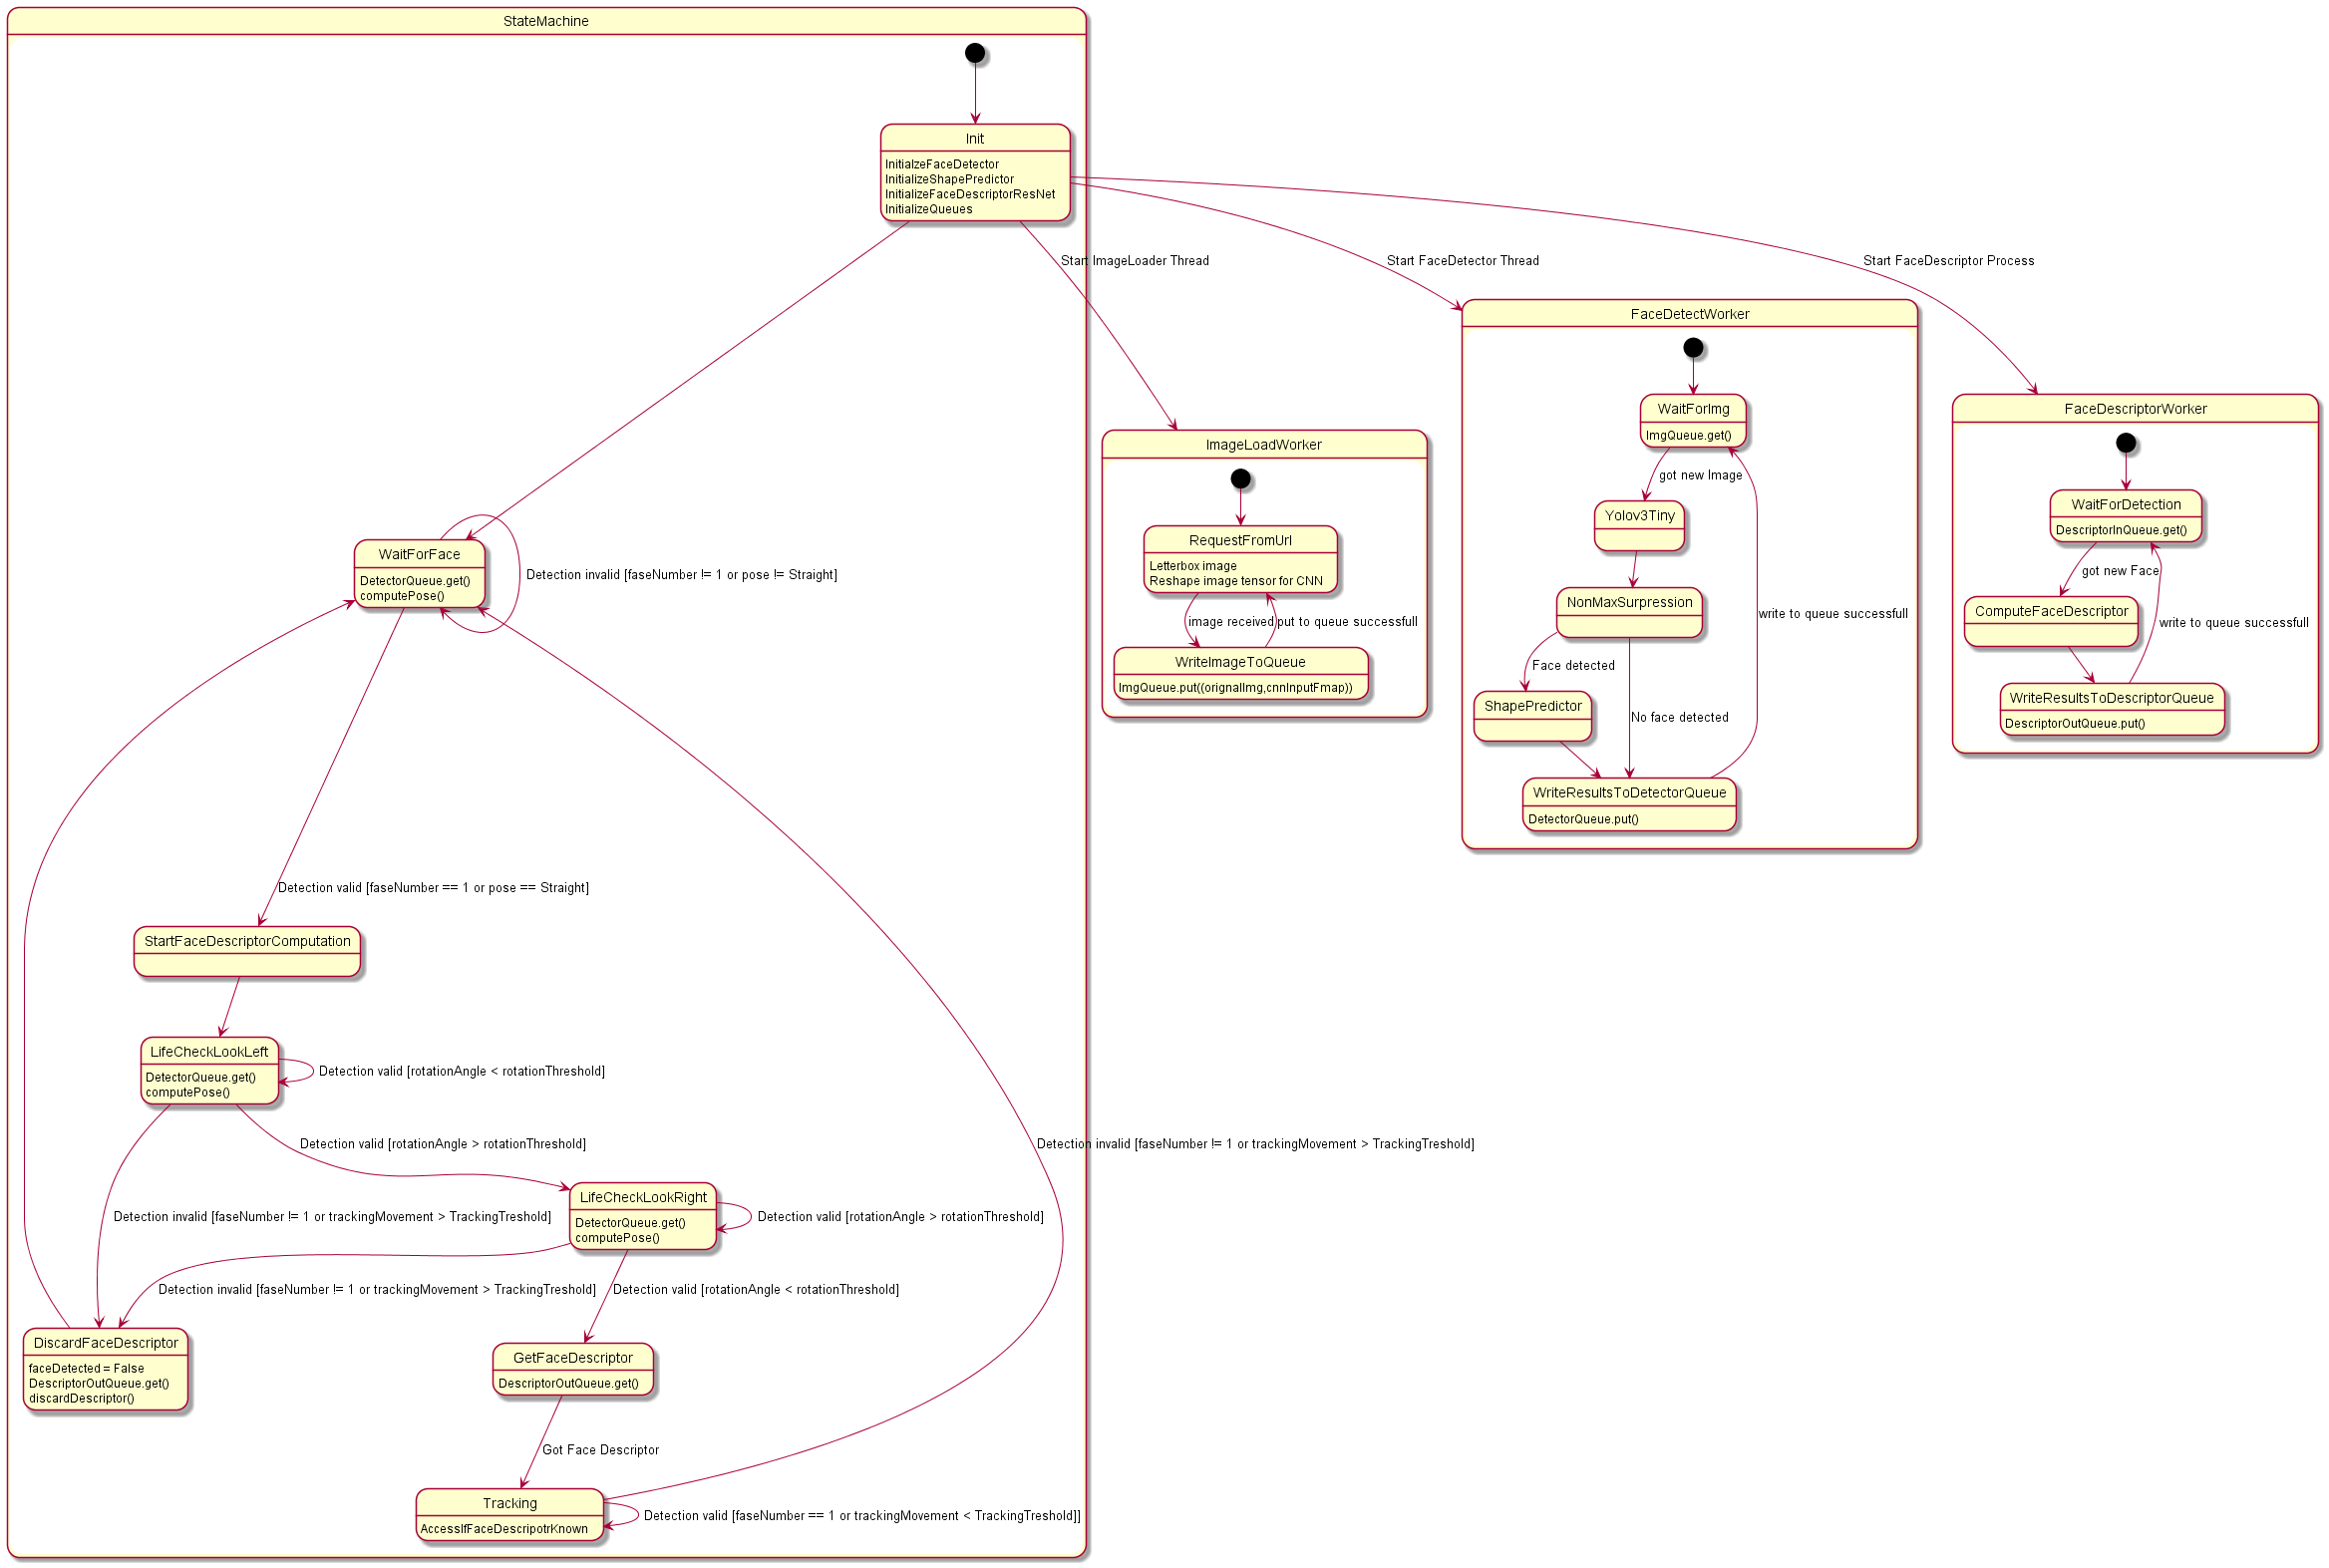
\includegraphics[width=1.5\textwidth]{../sources/graphics/StateMachine.png}
		\caption[Face verification system algorithm]{Face verification system algorithm. Main state machine and workers for loading an image, for detection faces and landmarks and for computing the face descriptor.}
		\label{fig:statemachine}
	\end{figure} 
\end{landscape}
The FaceDescriptorWorker is started as a process. That has the benefit that the execution of the FaceDescriptorWorker can be done in parallel on the second \gls{CPU} of the ARM Cortex A9 processor. The FaceDescriptorWorker gets the detected face from the DescriptorInQueue, processes the face descriptor, and writes the results into the DescriptorOutQueue. However, the state puts only newly detected faces into the DescriptorInQueue. \\
\\\
After initializing the background workers, the state machine changes into the WaitForFace state. In that state, the face verification system waits until a single face that is looking straight into the camera is detected. If that is fulfilled, it changes to the StartDescriptorComputationState, which puts the detected face into the DescriptorInQueue. That triggers the FaceDescriptorWorker to start computing the face descriptor and putting it into the DescriptorOutQueue. \\
In parallel to the face descriptor computation, the liveness starts by changing into the LiveCheckLookLeft state. The user interface prompts the user to look to the left. When the computed rotation angle exceeds the given threshold, the state machine changes the LiveCheckLookRight state. The user interface prompts the user to look to the right. If the computed rotation angle exceeds the threshold, the liveness check is successful, and the state machine changes into the GetFaceDescriptor state. \\
If the face verification system recognizes no face or more than one face during the liveness check, the face descriptor is discarded and the face verification system restarts in the WaitForFace state. The same happens when the movement of the face exceeds the given threshold. \\
In the GetFaceDescriptor state, the face verifications system checks if the computation of the face descriptor is already done by checking the DescriptorOutQueue. If the computation is done it changes into the tracking state, otherwise it keeps on waiting for the face descriptor. \\
In the tracking state, the system tracks the face and falls back to the WaitForFace state if the tracking fails. In this state, the system has a face descriptor from a verified living person who looks into the camera. That information can then be used for further steps. For example, it can be checked whether this person is already registered and if access is granted.

\chapter{Results}
\begin{figure}[h]
	\centering
	\includesvg[width=\textwidth]{../sources/graphics/timing.svg}
	\caption[Timing of the threads and processes of the implemented application.]{Timing of the threads and processes of the implemented application.}
	\label{fig:timing}
\end{figure} 

\begin{table}[h]
	\centering
	\begin{tabular}{lll}
		\toprule[1.5pt]
		\textbf{Thread/Process} & \textbf{Subtask}  & \textbf{execution time}  \\
		\midrule[1.5pt] 
		\multirow{ 2}{*}{\textbf{StateMachine}}	& Do state actions			& variable \\ 
				 						& Plot to screen			& 2.5\si{ms} \\ 
		\multirow{ 2}{*}{\textbf{ImageLoader}} 	& Load image from IP cam	& 263\si{ms}\\
										& Prepare image for CNN		& 7\si{ms}\\
		\multirow{ 2}{*}{\textbf{Detector}} 		& YOLOv3-tiny + \gls{nms}	& 150\si{ms}\\	
										& Predict Landmarks			& 29\si{ms}\\
		FaceDescriptor					& Compute face descriptor	& 5\si{s}	\\	
		\bottomrule[1.5pt]
	\end{tabular}
	\caption{Execution time of threads, processes and subtasks.}	
	\label{tab:execution-times}
\end{table}
\Cref{fig:timing} visualizes the timing of the threads and processes of the implemented application. It visualizes the parallel execution of loading images, detecting faces, computing the face descriptor and the state machine. \Cref{tab:execution-times} gives an overview of the execution times of the threads, processes, and their subtasks. \Cref{fig:timing} and \Cref{tab:execution-times} show that the minimum time for verifying a face is approximately 5.5\si{s}. That time includes the liveness check and the computation of the face descriptor. The face verification system achieves a frame rate of 3\si{fps} for loading an image from the IP camera, detecting faces, predicting the landmarks, computing the pose of the face, and plotting the results to the screen.  \\ 
\\\
The face verification system achieves an accuracy of 99.38\% for identifying faces when using a distance threshold of 0.6. The accuracy is determined using the LFW benchmark. The face detection achieves an accuracy of 0.986\% when using a reduced version of the vgg-dataset. However, the vgg-dataset has the drawback that most images have a perfect illumination, which makes the face detection sensitive to illumination. \\
\\\
For the face verification system, the memory clock, as well as the processing element clock of the Intuitus hardware accelerator, use a clock frequency of 100\si{MHz}. That leads to a sufficient inference time of the YOLOv3 CNN of 112\si{ms} and low power consumption of the used Zybo-Z7-20 board of approximately 3.3\si{W}. That leads to an energy consumption of 1\si{Ws} for a single face detection and an energy consumption 18.15\si{Ws} for verifying a face. 



\chapter{Conclusion}
Face verification can be a reliable alternative to keys and passwords since new deep neural network based solutions offer high accuracy. However, the computations required for processing the neural networks lead to high power consumption, that should be avoided, especially in times of climate change.\\
\\\
For this reason, this work shows how to create a power-efficient face verification system in an \gls{FPGA} device. It uses the Intuitus hardware accelerator for detecting faces with an accuracy of  0.986\% and the \gls{CPU} of the Zynq device for computing facial landmarks and the face descriptor, which achieves an accuracy of $99.38\%$ using the LFW benchmark. The presented implementation achieves a frame rate of 3\gls{fps} and requires a minimum of 5.5\si{s} for doing a liveness check and for computing the face descriptor. \\
The face verification system has a power consumption of 3.3\si{W}. That leads to an energy dissipation of 1\si{Ws} per face detection and 18.15\si{Ws} for doing a single face verification. 

\chapter{Outlook}
Basically, the execution speed of the face descriptor ResNet on the CPU is sufficient for the given task. However, an acceleration of the calculations by the FPGA would make sense as several face descriptors could be calculated for different facial poses of a face, thereby increasing the reliability considerably. \\
In addition, it would make sense to retrain the face recognition using a more complex dataset that includes images with different illuminations to reduce the illumination sensitivity. For example, the labeled faces in the wild (LFW) dataset can be used for retraining the face descriptor. \\
Another possible improvement would be to use an additional camera to see the face from a different angle and thereby make it almost impossible to trick the face verification system by showing an image or a video to the camera. 

	
	
	

	%----------------------------------------------------------------------------
	%
	%
	%----------------------------------------------------------------------------
	%
	% Bibliography
	%
	%\backmatter
	%\printbibliography
	%\bibliographystyle{../sources/classes-styles/IEEEtran}
	%\bibliography{../sources/bibliography/bibliography}
	% uncomment the following line if you want the bibliography be shown in table of contents
	%\addcontentsline{toc}{chapter}{Bibliography}
	
	% Appendix
	%
	
\end{document}
%
%----------------------------------------------------------------------------

%%% Local Variables:
%%% mode: latex
%%% TeX-master: t
%%% End:
